Community detection is the problem of identifying subsets of vertices that exhibit higher connectivity among themselves than with the rest of the network. The identified communities are intrinsic when based on network topology alone, and are disjoint when each vertex belongs to only one community. These communities, also known as clusters, shed light on the organization and functionality of the network. It is an NP-hard problem with applications in topic discovery, protein annotation, recommendation systems, and targeted advertising \cite{com-gregory10}.\ignore{One of the difficulties in the community detection problem is the lack of apriori knowledge on the number and size distribution of communities \cite{com-blondel08}.} The Louvain method \cite{com-blondel08} is a popular heuristic-based approach for community detection. It employs a two-phase approach, comprising a local-moving phase and an aggregation phase, to iteratively optimize the modularity metric --- a measure of community quality \cite{com-newman06}.

Despite its popularity, the Louvain method has been observed to produce internally-disconnected and badly connected communities. To address these shortcomings, Traag et al. \cite{com-traag19} propose the Leiden algorithm. It introduces an additional refinement phase between the local-moving and aggregation phases. The refinement phase allows vertices to explore and potentially form sub-communities within the communities identified during the local-moving phase. This enables the Leiden algorithm to identify well-connected communities \cite{com-traag19}.

However, applying the original Leiden algorithm to massive graphs has raised computational bottlenecks, mainly due to its inherently sequential nature --- similar to the Louvain method \cite{com-halappanavar17}. In contexts where scalability is paramount, the development of an optimized parallel Leiden algorithm becomes imperative --- especially in the multicore/shared memory setting, due to its energy efficiency and the prevalence of hardware with large memory sizes.

This technical report addresses precisely this challenge by presenting a parallel implementation of the Leiden algorithm, targeting both quality and efficiency. Existing studies on parallel Leiden algorithm propose a number of parallelization techniques, but do not address optimization for the aggregation phase of the Leiden algorithm \cite{verweijfaster}, which emerges as a bottleneck after the local-moving phase of the algorithm has been optimized. In addition, a number of optimization techniques that apply to the Louvain method also apply to the Leiden algorithm.\ignore{However, these are scattered over a number of papers, making it difficult for a reader to get a grip over them.}

%% Introduction for Leiden algorithm
%% Problems with Louvain: Internally disconnected communities
% Louvain algorithm may identify communities that are internally disconnected. A certain node that acts as bridge may move to another community. Remaining vertices stay well connected. This occurs frequently in practice. Iterating the algorithm aggravates the problem. Although its does not decrease quality function.


%% Problems with Louvain: Arbitrarily badly connected communities
% Further, Louvain algorithm may identify communities that are arbitrarily badly connected. Nodes that are grouped together may be better off split into multiple communities, i.e., splitting the community can improve the quality. This is not the same as resolution limit problem with modularity, that causes small communities to be clustered with large communities. Louvain only guarantees that no communities can be merged (well separated). Badly connected => Leiden could split given communities.


%% Leiden algorithm
% Unlike the Louvain algorithm, the Leiden algorithm has an additional refine phase after the local-moving phase, where nodes within each community are local-moved again after reset. Refine phase is randomized (not greedy), the community a node moves to is proportional to the delta-modularity of moving to that community. When nodes are greedily moved, some optimal partitions cannot be found. It uses local-move with pruning (however, we apply this optimizations to both algorithms).


%% Leiden algorithm: Guarantees
% 1. All communities are $\gamma$-separated.
% 2. All communities are $\gamma$-connected.
% If partition didn’t change:
% 3. All nodes are optimally assigned.
% 4. All communities are subpartition $\gamma$-dense.
% 5. All communities are uniformly $\gamma$-dense.
% 6. All communities are subset optimal.


%% Idea behind Leiden algorithm
% The idea behind the new leiden algorithm is that louvain can find arbitrarily badly connected communities and even disconnected communities. Louvain algorithm has two phases, a locl-moving phase, and an aggregation phase (for each pass). Leiden algorithm adds another refinement phase between the two, where it allows vertices to find sub-communities within the communities just obtained from local-moving phase.


%% Came across Leiden algorithm
% I came across this paper on Leiden method which shows that some communities produced by Louvain method are badly connected, and some even disconnected (and why this is not good). Louvain method relies on modularity score, which has resolution issues (cant handle too small communities, solution CPM score). They add a refinement step and a better (random) local move approach. The restructuring phase is also with refinement. They also proved is supplementary section why its better.
% https://www.nature.com/articles/s41598-019-41695-z

% In both:
% Phase 1: Iterate until the score no longer improves (but Leiden can still proceed, maybe because its random)
% Phase 2: Form its smaller super-nodes graph
% Repeat until score no longer improves


%% More about Leiden algorithm
% - Separating disconnected communities
% Louvain algorithm may place diconnected groups of vertices within the same community. We could try disconnecting them either at the end or at the end of each phase.
% - Dynamic Leiden algorithm
% This involves applying a refinement phase after the local-moving phase of the Louvain algorithm. It also should be able to handle community split without a call to Static Louvain/Leiden.
% In the end we can measure the quality of communities obtained through our disconnected Louvain and dynamic Leiden in terms of quality, stability, and performance.





\subsection{Our Contributions}

This report introduces GVE-Leiden\footnote{https://github.com/puzzlef/leiden-communities-openmp}, an optimized parallel implementation of the Leiden algorithm for community detection on shared memory multicores. On a machine with two 16-core Intel Xeon Gold 6226R processors, GVE-Leiden achieves a processing rate of $352 M$ edges/s on a $3.8 B$ edge graph, and outperforms the original Leiden implementation, igraph Leiden, and NetworKit Leiden by $373\times$, $86\times$, and $7.2\times$ respectively, while identifying communities of the same quality as the first two implementations, and $26\%$ higher quality than NetworKit. Compared to GVE-Louvain, our optimized parallel Louvain implementation, GVE-Leiden achieves an $11$-fold reduction in internally-disconnected communities, with only a $36\%$ increase in computation time. With doubling of threads, GVE-Leiden exhibits an average performance scaling of $1.6\times$. This makes GVE-Leiden an attractive choice for high-quality community detection on massive graphs.




%% - Use --- for a dash.
%% - Use ``camera-ready'' for quotes.
%% - Use {\itshape very} or \textit{very} for italicized text.
%% - Use \verb|acmart| or {\verb|acmart|} for mono-spaced text.
%% - Use \url{https://capitalizemytitle.com/} for URLs.
%% - Use {\bfseries Do not modify this document.} for important boldface details.
%% - Use \ref{fig:name} for referencing.

%% For a block of pre-formatted text: 
% \begin{verbatim}
%   \renewcommand{\shortauthors}{McCartney, et al.}
% \end{verbatim}

%% For a list of items:
% \begin{itemize}
% \item the ``ACM Reference Format'' text on the first page.
% \item the ``rights management'' text on the first page.
% \item the conference information in the page header(s).
% \end{itemize}

%% For a table:
% \begin{table}
%   \caption{Frequency of Special Characters}
%   \label{tab:freq}
%   \begin{tabular}{ccl}
%     \toprule
%     Non-English or Math&Frequency&Comments\\
%     \midrule
%     \O & 1 in 1,000& For Swedish names\\
%     $\pi$ & 1 in 5& Common in math\\
%     \$ & 4 in 5 & Used in business\\
%     $\Psi^2_1$ & 1 in 40,000& Unexplained usage\\
%   \bottomrule
% \end{tabular}
% \end{table}

%% For a full-width table:
% \begin{table*}
%   \caption{Some Typical Commands}
%   \label{tab:commands}
%   \begin{tabular}{ccl}
%     \toprule
%     Command &A Number & Comments\\
%     \midrule
%     \texttt{{\char'134}author} & 100& Author \\
%     \texttt{{\char'134}table}& 300 & For tables\\
%     \texttt{{\char'134}table*}& 400& For wider tables\\
%     \bottomrule
%   \end{tabular}
% \end{table*}


%% For inline math:
% \begin{math}
%   \lim_{n\rightarrow \infty}x=0
% \end{math},

%% For a numbered equation:
% \begin{equation}
%   \lim_{n\rightarrow \infty}x=0
% \end{equation}

%% For an unnumbered equation:
% \begin{displaymath}
%   \sum_{i=0}^{\infty} x + 1
% \end{displaymath}

%% For a figure:
% \begin{figure}[h]
%   \centering
%   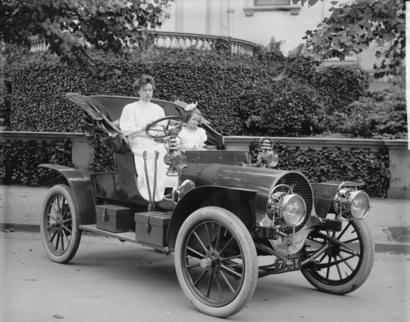
\includegraphics[width=\linewidth]{inc/sample-franklin}
%   \caption{1907 Franklin Model D roadster. Photograph by Harris \&
%     Ewing, Inc. [Public domain], via Wikimedia
%     Commons. (\url{https://goo.gl/VLCRBB}).}
%   \Description{A woman and a girl in white dresses sit in an open car.}
% \end{figure}

%% For a teaser figure.
% \begin{teaserfigure}
%   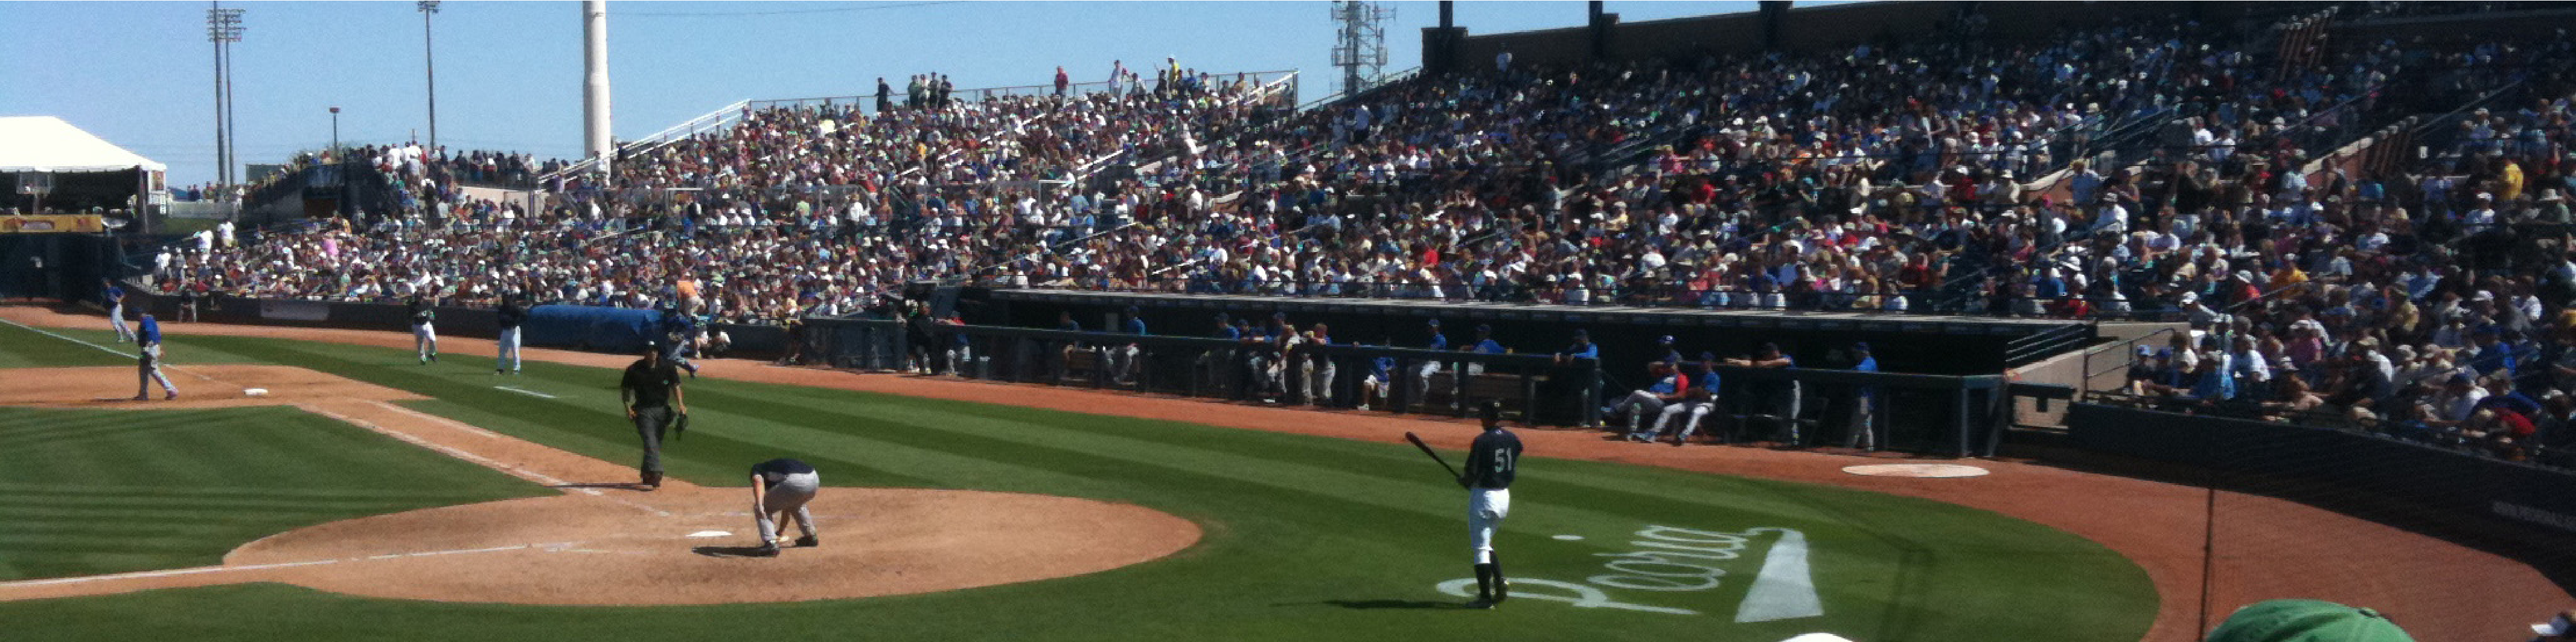
\includegraphics[width=\textwidth]{sampleteaser}
%   \caption{figure caption}
%   \Description{figure description}
% \end{teaserfigure}
